\chapter[বিজনেস ইন্টেলিজেন্স ড্যাশবোর্ড ও সিদ্ধান্ত-সহায়তা]{বিজনেস ইন্টেলিজেন্স ড্যাশবোর্ড ও\\ সিদ্ধান্ত-সহায়তা}\label{ch:dashboard}

\section{নকশার লক্ষ্য}
ড্যাশবোর্ড হলো সেই জায়গা যেখানে কাঠামোটি এর ব্যবহারকারী, অর্থাৎ বিক্রয়, সাপ্লাই-চেইন ও ঊর্ধ্বতন ব্যবস্থাপকদের সঙ্গে মিলিত হয়।
\citet{few2013} অনুসরণ করে এটি পাঁচটি প্রয়োজন পূরণের জন্য নকশা করা হয়েছে:
\begin{enumerate}
  \item \textbf{এক নজরে KPI}: ওভারভিউ পাতার শীর্ষে নিট বিক্রয়, ইউনিট, অর্ডার, গড় অর্ডার-মূল্য, ডিসকাউন্ট হার ও বছরের-শুরু-থেকে প্রবৃদ্ধি;
  \item \textbf{সামঞ্জস্যপূর্ণ ফিল্টার}: এক সেট ফিল্টার (বছর, অঞ্চল, চ্যানেল, গ্রাহকের ধরন, ক্যাটাগরি) সব পাতায় প্রযোজ্য;
  \item \textbf{তিনটি ব্যবস্থাপনা প্রশ্ন}: পাতাগুলো \emph{কী ঘটেছে} (ওভারভিউ, প্রবণতা, পণ্য, বাজার) থেকে \emph{কেন} (চালিকাশক্তি,
        বিভাগ) এবং \emph{সামনে কী} (পূর্বাভাস, অস্বাভাবিকতা, সুপারিশ) পর্যন্ত এগোয়;
  \item \textbf{সৎ উপস্থাপন}: পূর্বাভাস সবসময় পূর্বাভাস-ব্যবধানসহ দেখানো হয়, মডেলের নির্ভুলতা ব্যবহারকারীর কাছে দৃশ্যমান, এবং রং কেবল
        অর্থ বোঝাতে ব্যবহৃত;
  \item \textbf{বিনামূল্যে ও সহজলভ্য}: ড্যাশবোর্ড যেকোনো ওয়েব ব্রাউজারে চলে এবং বিনা খরচে হোস্ট করা হয়।
\end{enumerate}

\section{বাস্তবায়ন}
ড্যাশবোর্ডটি Streamlit ও Plotly দিয়ে একটি একক Python ফাইলে (\path{dashboard/app.py}) তৈরি। এটি 500,000টি কাঁচা সারি পড়ে না, বরং
পাইপলাইনের তৈরি সংক্ষিপ্ত সমষ্টিগত ডেটা পড়ে: অঞ্চল $\times$ চ্যানেল $\times$ গ্রাহকের ধরন $\times$ ক্যাটাগরি অনুযায়ী একটি মাসিক
কিউব, পণ্য-বাই-অঞ্চল মাসিক মোট, পূর্বাভাস, মডেল-স্কোর, বিভাগ-সারণি ও অস্বাভাবিকতার তালিকা। এদের মোট আকার প্রায় 2~MB, তাই বিনামূল্যের
হোস্টিংয়ে অ্যাপটি কয়েক সেকেন্ডে চালু হয়, অথচ প্রতিটি ফিল্টার-সমন্বয় নির্ভুল থাকে। প্রথমবার লোডের পর ডেটা মেমোরিতে cache থাকে।
\Cref{tab:pages}-এ নয়টি পাতার তালিকা।

\begin{table}[htbp]\centering\small
\caption{ইন্টারঅ্যাকটিভ ড্যাশবোর্ডের পাতাসমূহ}\label{tab:pages}
\begin{tabularx}{\linewidth}{@{}lX@{}}
\toprule
\textbf{পাতা} & \textbf{বিষয়বস্তু} \\ \midrule
Executive overview & KPI কার্ড, চলমান গড়সহ মাসিক বিক্রয়, ক্যাটাগরি, অঞ্চল ও চ্যানেলের মিশ্রণ, বার্ষিক সারণি \\
Trends \& seasonality & যেকোনো মাত্রায় স্তূপীকৃত প্রবণতা, বছর $\times$ মাস heat map, মৌসুমি সূচক, বছর-বনাম-বছর রেখা \\
Products \& portfolio & শীর্ষ-$N$ পণ্য, Pareto/ABC বিশ্লেষণ, ML পণ্য-বিভাগ, একক পণ্যের বিস্তারিত \\
Markets \& customers & অঞ্চল $\times$ চ্যানেল heat map, গ্রাহকের ধরন, আঞ্চলিক CAGR, ML বাজার-বিভাগ \\
Demand forecast & ব্যবধানসহ 12-মাসের দৃষ্টিভঙ্গি, ক্যাটাগরি ও পণ্যের পূর্বাভাস, মডেল লিডারবোর্ড, CSV ডাউনলোড \\
Machine-learning models & feature importance-সহ রিগ্রেশন, ক্লাসিফিকেশন ও ক্লাস্টারিংয়ের ফলাফল \\
Anomaly monitor & প্রত্যাশিত স্তরের বিপরীতে দৈনিক বিক্রয় ও চিহ্নিত দিন; সবচেয়ে সন্দেহজনক অর্ডার \\
Insights \& recommendations & করণীয়সহ স্বয়ংক্রিয়ভাবে তৈরি অন্তর্দৃষ্টি \\
Data quality \& method & যাচাই-প্রতিবেদন, পরিষ্কারকরণের লগ ও স্থাপত্যের চিত্র \\ \bottomrule
\end{tabularx}
\end{table}

\begin{figure}[htbp]\centering
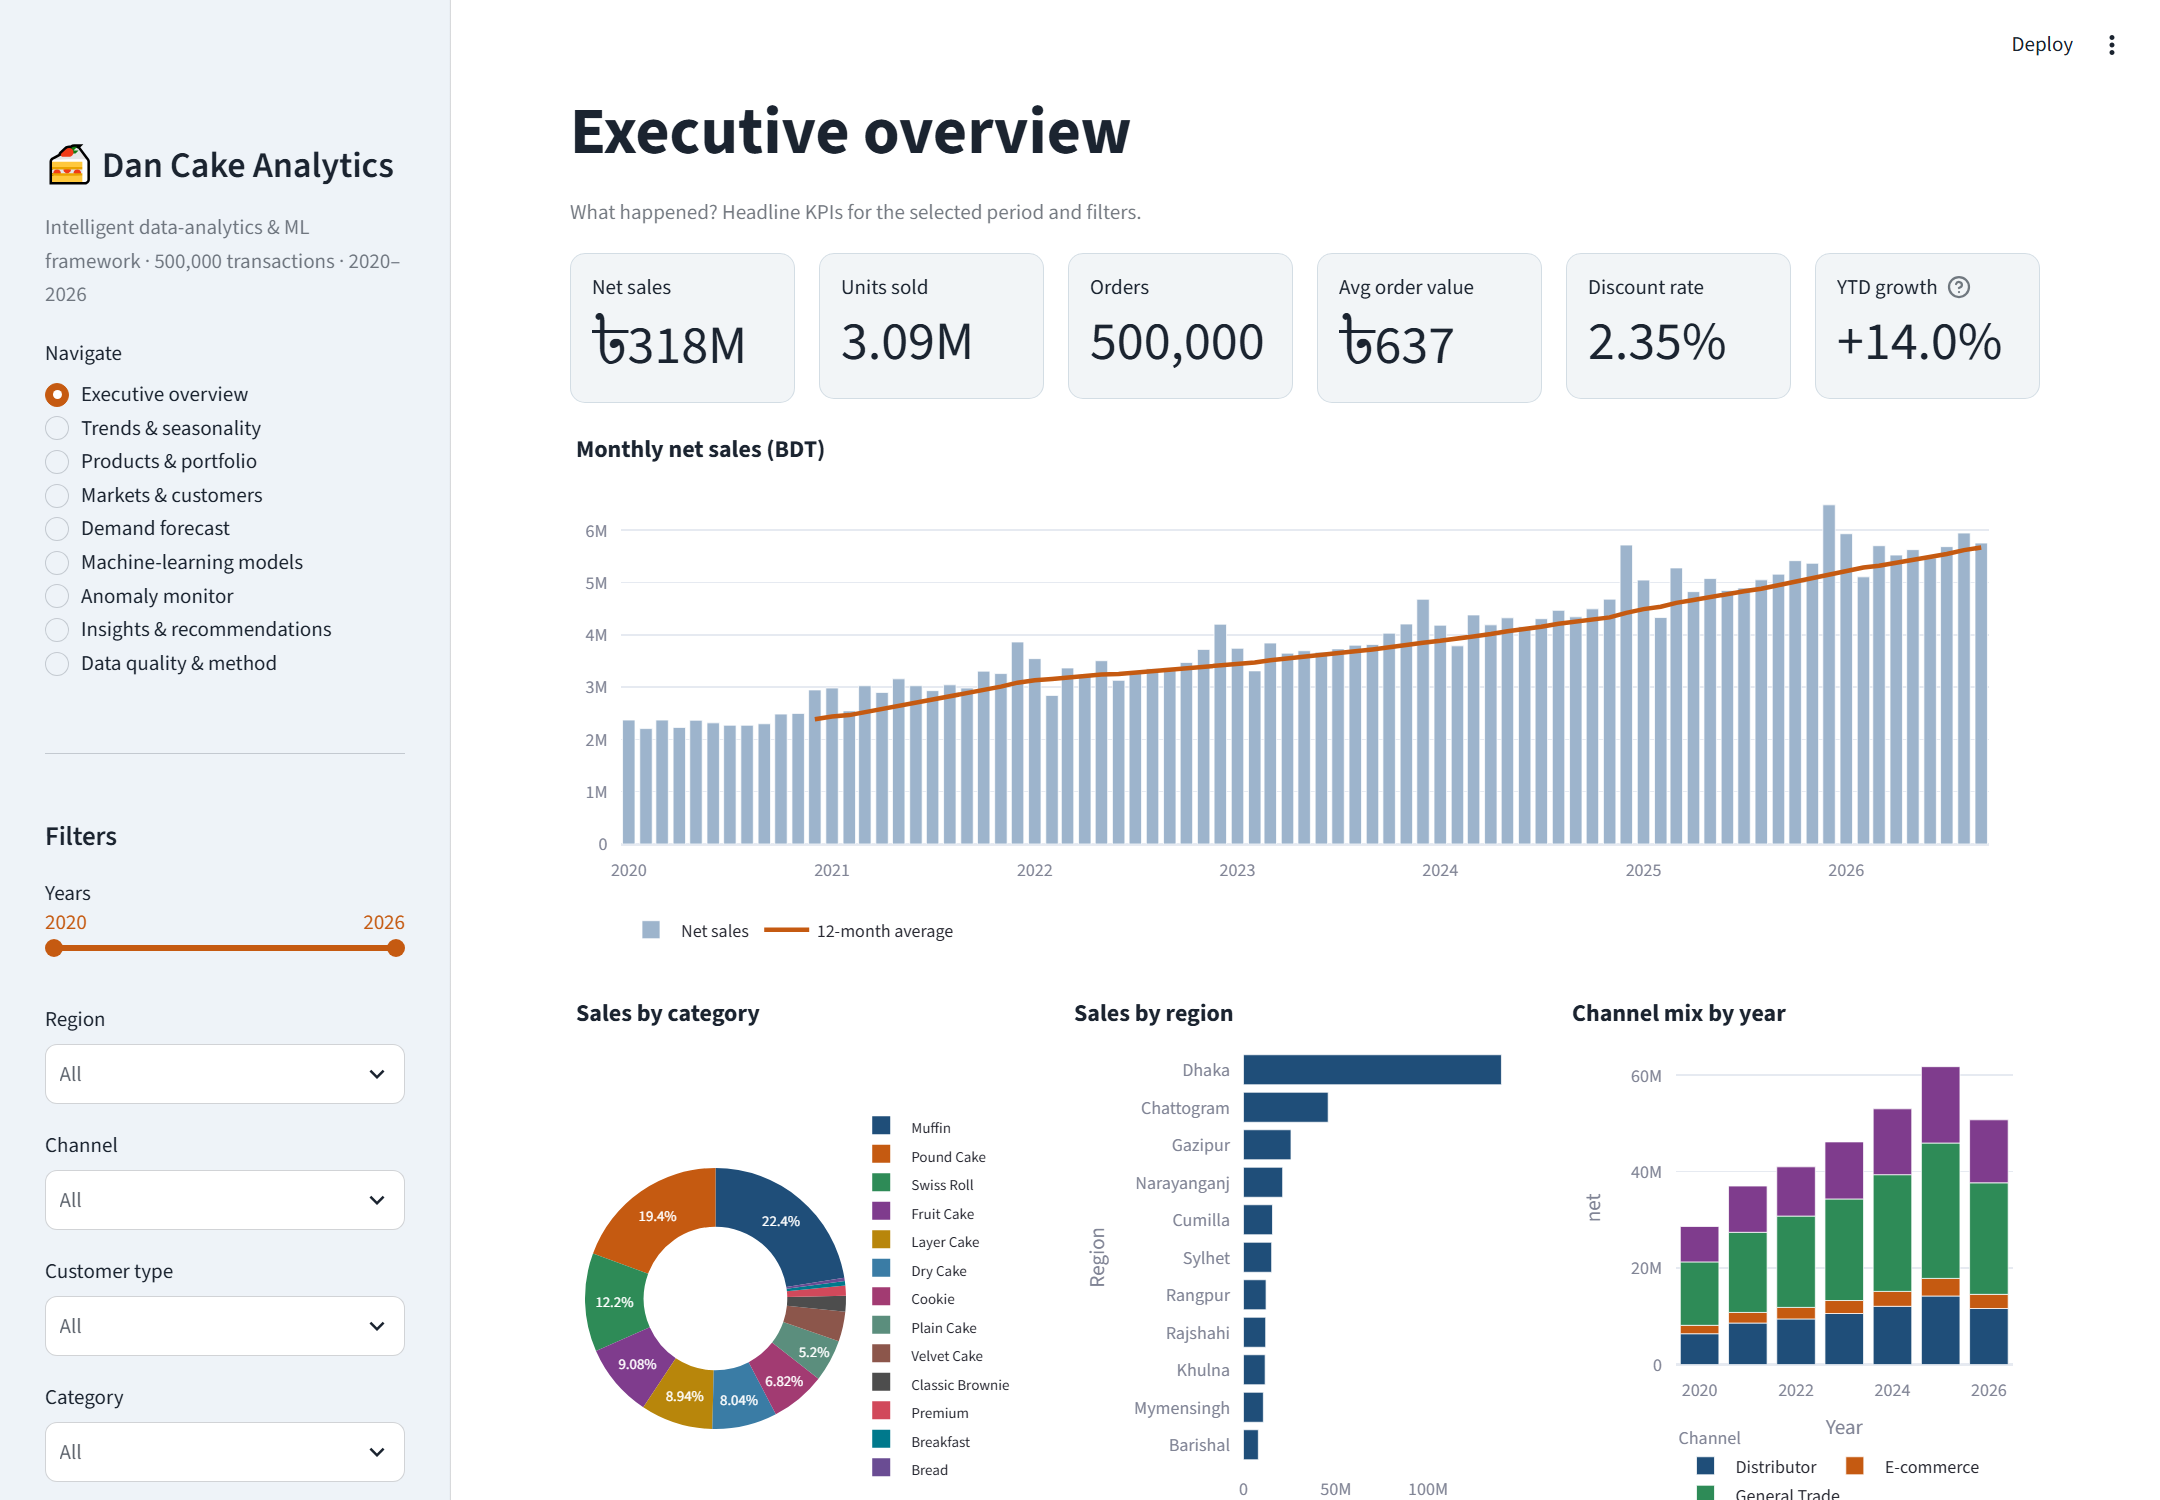
\includegraphics[width=\linewidth]{dash_overview}
\caption{ড্যাশবোর্ডের Executive overview পাতা}\label{fig:dashoverview}
\end{figure}

\begin{figure}[htbp]\centering
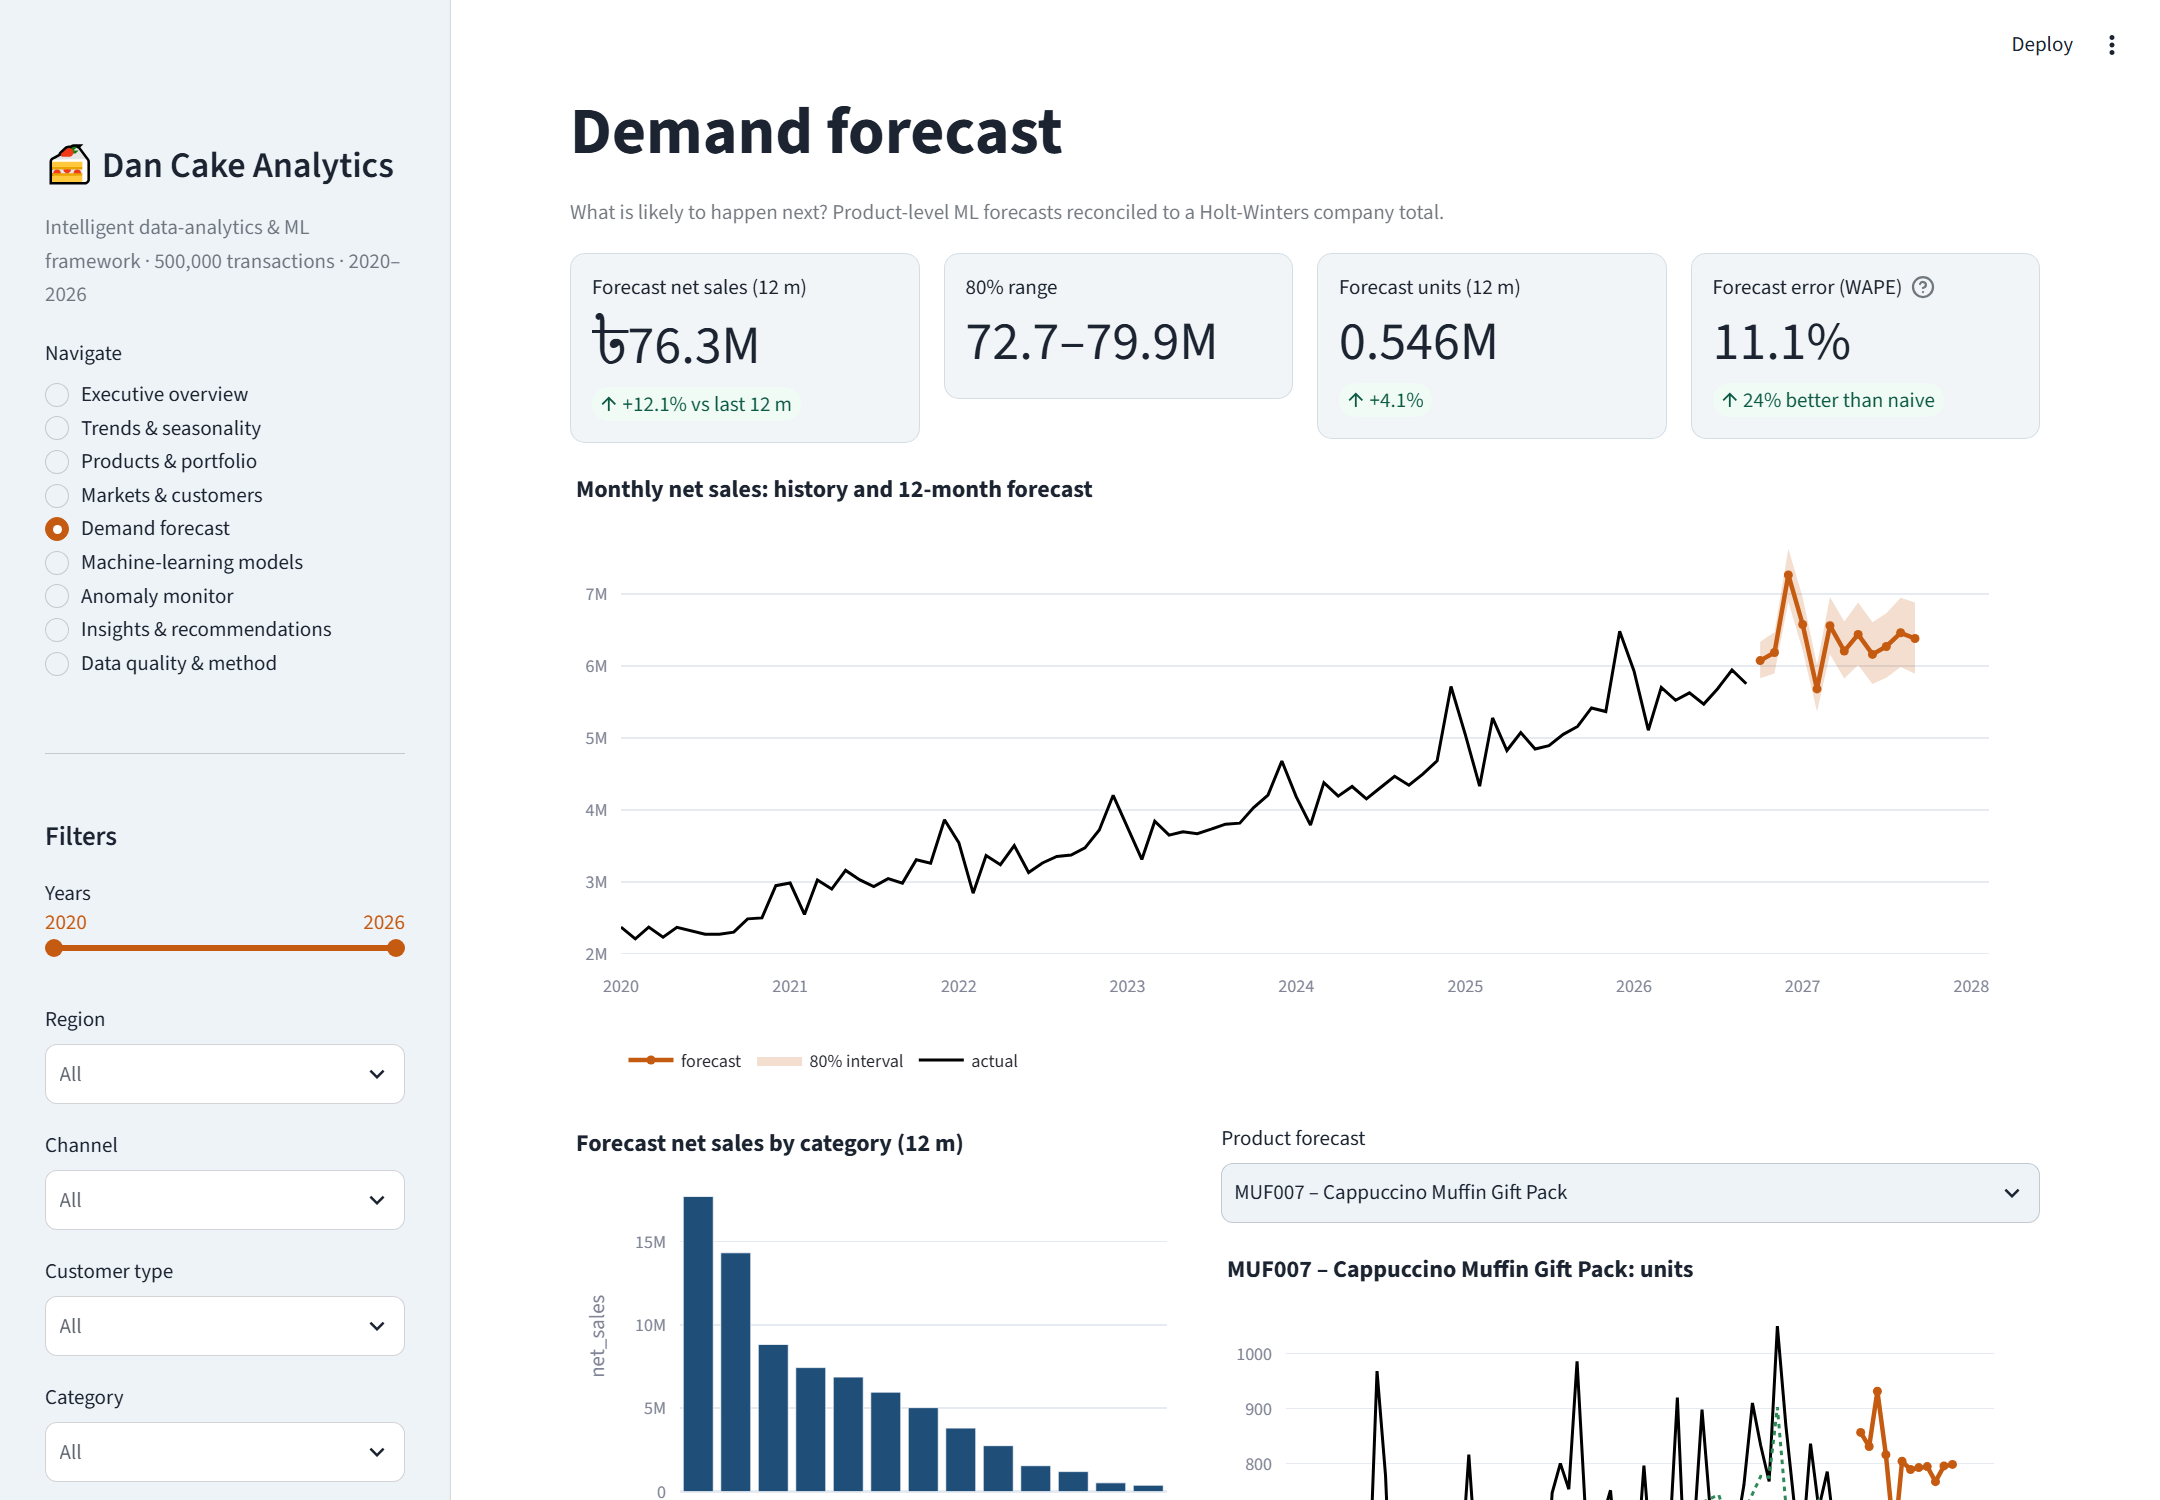
\includegraphics[width=\linewidth]{dash_forecast}
\caption{ড্যাশবোর্ডের চাহিদা-পূর্বাভাস পাতা: 80\% ব্যবধানসহ 12-মাসের দৃষ্টিভঙ্গি}\label{fig:dashforecast}
\end{figure}

\section{প্রকাশ}
দুটি বিনামূল্যের ওয়েব সেবা প্রস্তুত করা হয়েছে:
\begin{itemize}
  \item \textbf{ইন্টারঅ্যাকটিভ ড্যাশবোর্ড}, যা প্রকল্পের GitHub রিপোজিটরি থেকে সরাসরি Streamlit Community Cloud-এ প্রকাশিত
        (ঠিকানার ধরন \dashurl);
  \item একটি \textbf{প্রকল্প ওয়েবসাইট}, \texttt{website.py} দিয়ে তৈরি একটি স্থির পাতা যা GitHub Pages থেকে পরিবেশিত (\siteurl)। এটি
        ইন্টারঅ্যাকটিভ Plotly চার্টসহ প্রকল্পের সারসংক্ষেপ দেয় এবং ড্যাশবোর্ড, সোর্স কোড ও এই প্রতিবেদনের লিংক দেয়।
\end{itemize}
দুটি সেবাই বিনামূল্যে একটি HTTPS সাব-ডোমেইন দেয়। পরে একটি নিজস্ব ডোমেইন কেনা হলে কোড না বদলেই DNS \texttt{CNAME} রেকর্ডের মাধ্যমে তা
GitHub Pages-এ যুক্ত করা যায়। ধাপে ধাপে প্রকাশের পদ্ধতি \cref{app:reproduce}-এ দেওয়া আছে।

\section{সিদ্ধান্ত-সহায়ক স্তর}
শেষ স্তরটি মডেলের ফলাফলকে সুপারিশে রূপান্তর করে। মডিউল \texttt{insights.py} মেট্রিক ফাইলগুলো পড়ে বাক্য-টেমপ্লেটে বর্তমান ফলাফল
বসায়, তাই নতুন ডেটা প্রক্রিয়া হলে প্রতিটি অন্তর্দৃষ্টি হালনাগাদ থাকে এবং কোনোটিই হাতে লেখা হয় না। এই ডেটাসেটের জন্য তৈরি অন্তর্দৃষ্টিগুলো:

\begin{enumerate}[leftmargin=*,itemsep=4pt]
\item \textbf{প্রবৃদ্ধি (কী ঘটেছে)।} 2020 থেকে 2025 পর্যন্ত নিট বিক্রয় বছরে 16.6\% হারে বেড়েছে, কিন্তু ইউনিট বেড়েছে মাত্র 5.0\%; গড়ে বার্ষিক প্রবৃদ্ধির 11.3 শতাংশ-বিন্দু এসেছে মূল্য ও মিশ্রণ থেকে এবং 5.0 পরিমাণ থেকে। \emph{সুপারিশ:} পরিমাণ-প্রবৃদ্ধিকে আলাদা KPI হিসেবে অনুসরণ করুন; মূল্য-নির্ভর প্রবৃদ্ধি অনির্দিষ্টকাল টেকসই নয়।
\item \textbf{মূল্য নির্ধারণ (কেন ঘটেছে)।} পণ্য, বছর ও মৌসুম নিয়ন্ত্রণ করার পর চাহিদার নির্ণীত মূল্য-স্থিতিস্থাপকতা +0.09 (95\% CI -0.28 থেকে +0.46), যা শূন্য থেকে তাৎপর্যপূর্ণভাবে আলাদা নয়। ডিসকাউন্টের সঙ্গে অর্ডারের আকারের কোনো সম্পর্ক নেই (Spearman rho = 0.001)। \emph{সুপারিশ:} ডিসকাউন্ট বাজেট পুনর্বিবেচনা করুন (এই সময়কালে 7.7 মিলিয়ন টাকা): ডিসকাউন্ট বিক্রির পরিমাণ বাড়ায় বলে মনে হয় না।
\item \textbf{মৌসুমিতা (কী ঘটেছে)।} ডিসেম্বর শীর্ষ মাস (সূচক 125, গড় মাস = 100) এবং ফেব্রুয়ারি সবচেয়ে দুর্বল (86)। মৌসুমি প্রভাব পরিসংখ্যানিকভাবে শক্তিশালী (Kruskal-Wallis p < 0.001)। \emph{সুপারিশ:} অক্টোবর থেকে মজুদ ও ডিস্ট্রিবিউটর-সক্ষমতা বাড়ান; ফেব্রুয়ারিতে প্রমোশন ও রক্ষণাবেক্ষণের পরিকল্পনা করুন।
\item \textbf{পোর্টফোলিও (কী ঘটেছে)।} Muffin সবচেয়ে বড় ক্যাটাগরি (বিক্রয়ের 22.4\%); 52টি পণ্যের শীর্ষ 10টি আয়ের 38.5\% দেয় এবং 27টি পণ্য `A' শ্রেণি (বিক্রয়ের 80\%) গঠন করে। \emph{সুপারিশ:} প্রথমে A-শ্রেণির পণ্যের প্রাপ্যতা নিশ্চিত করুন; C-শ্রেণির পণ্য যৌক্তিকীকরণ বা পুনঃস্থাপনের জন্য পর্যালোচনা করুন।
\item \textbf{পোর্টফোলিও (বিভাজন)।} ক্লাস্টারিং 5টি পণ্য-বিভাগ খুঁজে পেয়েছে; `Premium \& gift packs' সবচেয়ে দ্রুত বাড়ছে (বছরে ইউনিট +7.8\%, বিক্রয়ের 33.3\%)। \emph{সুপারিশ:} `Premium \& gift packs'-এর জন্য তাকের জায়গা ও বিপণনে অগ্রাধিকার দিন।
\item \textbf{বাজার (কী ঘটেছে)।} ঢাকা একাই বিক্রয়ের 43.9\% এবং ঢাকা ও চট্টগ্রাম মিলে 58.3\% আনে। General Trade সবচেয়ে বড় চ্যানেল (45.6\%), আর E-commerce 5.9\%। \emph{সুপারিশ:} দ্বিতীয় সারির শহর গড়ে তুলে এবং ছোট ভিত্তি থেকে বাড়তে থাকা E-commerce প্রসারিত করে কেন্দ্রীভবনের ঝুঁকি কমান।
\item \textbf{বাজার (বিভাজন)।} `Emerging high-growth cells' বিভাগটি (19টি অঞ্চল-চ্যানেল-গ্রাহক কোষ, মূলত Cumilla, Khulna, Mymensingh) বছরে +33.2\% হারে বাড়ছে, যা 4টি বাজার-বিভাগের মধ্যে দ্রুততম। \emph{সুপারিশ:} মাঠ-পর্যায়ের বিক্রয় ও ডিজিটাল বিপণনের প্রচেষ্টা এই উদীয়মান কোষগুলোতে বরাদ্দ করুন।
\item \textbf{অর্ডার (পূর্বাভাস)।} একটি অর্ডার বড় হবে কি না ($\geq$ 10 ইউনিট) তা মাঝারি মাত্রায় পূর্বাভাসযোগ্য (সেরা ROC-AUC 0.712, Logistic Regression); চ্যানেলই সবচেয়ে শক্তিশালী চালিকাশক্তি: ডিস্ট্রিবিউটর অর্ডারের 48\% বড়, অথচ অনলাইনে 8\%। \emph{সুপারিশ:} যানবাহন ও মজুদ বণ্টনে বড়-অর্ডার স্কোর ব্যবহার করুন, মূলত চ্যানেল-স্তরে।
\item \textbf{পূর্বাভাস (সামনে কী ঘটবে)।} Support Vector Regression মডেল পরের মাসের পণ্য-চাহিদা 11.1\% weighted ত্রুটিতে পূর্বাভাস করে, যা seasonal-naive নিয়মের চেয়ে 24\% কম RMSE। অক্টোবর 2026 থেকে সেপ্টেম্বর 2027-এর নিট বিক্রয়ের পূর্বাভাস 76.3 মিলিয়ন টাকা (আগের 12 মাসের চেয়ে +12.1\%; 80\% ব্যবধান 72.7 -- 79.9 মিলিয়ন টাকা)। \emph{সুপারিশ:} মাসিক উৎপাদন পরিকল্পনায় পণ্য-স্তরের পূর্বাভাস এবং নিরাপত্তা-মজুদে পূর্বাভাস-ব্যবধান ব্যবহার করুন।
\item \textbf{ঝুঁকি (অস্বাভাবিকতা)।} 2,465টি ব্যবসায়িক দিনের 28টি অস্বাভাবিক হিসেবে চিহ্নিত। একটি নিয়ন্ত্রিত পরীক্ষায় নিয়ম ও Isolation Forest মিলে রোপিত 1,000টি ডেটা-ত্রুটির 91\% ধরেছে। \emph{সুপারিশ:} প্রতিদিন অ্যানোমালি যাচাই চালান এবং মাস-শেষের প্রতিবেদনের আগে চিহ্নিত দিন ও অর্ডার তদন্ত করুন।
\end{enumerate}

প্রতিটি অন্তর্দৃষ্টিকে ক্ষেত্র ও যে ব্যবস্থাপনা প্রশ্নের উত্তর দেয় তা দিয়ে চিহ্নিত করা হয়েছে এবং একটি সুনির্দিষ্ট করণীয়ের সঙ্গে জোড়া দেওয়া হয়েছে।
ফলে ড্যাশবোর্ডটি কেবল প্রতিবেদন-টুল নয়, একটি \emph{সিদ্ধান্ত-সহায়ক ব্যবস্থা}।

\section{সিস্টেম মূল্যায়ন}
প্রস্তাবনায় সিস্টেমটিকে পূর্বাভাস-কর্মদক্ষতা, ব্যবহারযোগ্যতা, বিশ্লেষণী উপযোগিতা, ভিজ্যুয়ালাইজেশনের মান ও প্রক্রিয়াকরণ-দক্ষতায় মূল্যায়ন
করতে বলা হয়েছিল। \Cref{tab:syseval} প্রমাণগুলোর সারসংক্ষেপ দেয়।

\begin{table}[htbp]\centering\small
\caption{প্রস্তাবনার মানদণ্ডে কাঠামোর মূল্যায়ন}\label{tab:syseval}
\begin{tabularx}{\linewidth}{@{}lX@{}}
\toprule
\textbf{মানদণ্ড} & \textbf{প্রমাণ} \\ \midrule
পূর্বাভাস-কর্মদক্ষতা & সব ML পূর্বাভাসক naive বেঞ্চমার্ককে হারিয়েছে; সেরা WAPE \BestRegWAPE\%; কোম্পানি-পর্যায়ে MAPE \HWMAPE\%;
ক্লাসিফিকেশনে ROC-AUC \ClsAUC (\cref{ch:models}) \\
বিশ্লেষণী উপযোগিতা & প্রবৃদ্ধির মান, ডিসকাউন্টের অকার্যকারিতা, মৌসুমিতা, কেন্দ্রীভবনের ঝুঁকি, বিভাগ ও অস্বাভাবিকতা বিষয়ে অন্তর্দৃষ্টি, প্রতিটির সঙ্গে
করণীয় \\
ব্যবহারযোগ্যতা & এক সেট সর্বজনীন ফিল্টার; কাজভিত্তিক নয়টি পাতা; সহজ ভাষার ক্যাপশন; ডাউনলোডযোগ্য পূর্বাভাস; ইনস্টলেশন ছাড়াই যেকোনো
ব্রাউজারে চলে \\
ভিজ্যুয়ালাইজেশনের মান & Few-এর নীতি: KPI কার্ড, সাজানো বার, heat map, পূর্বাভাসে ব্যবধান, কোনো 3-D বা সাজসজ্জামূলক চার্ট নয়, সামঞ্জস্যপূর্ণ
রং \\
প্রক্রিয়াকরণ-দক্ষতা & \NRows সারির যাচাই ও পরিষ্কারকরণ 20 সেকেন্ডের কম সময়ে; ওয়্যারহাউস লোড \WarehouseSeconds সেকেন্ডে; মডেল টিউনিংসহ
পুরো পাইপলাইন একটি সাধারণ ল্যাপটপে প্রায় 20 মিনিটে; ড্যাশবোর্ড-ডেটা প্রায় 2 MB \\
পুনরুৎপাদনযোগ্যতা & একটি কমান্ডে সব ডেটা, মডেল, চিত্র, সারণি ও সংখ্যা পুনরায় তৈরি; নির্দিষ্ট random seed; স্বয়ংক্রিয় টেস্ট \\ \bottomrule
\end{tabularx}
\end{table}

ব্যবস্থাপকদের নিয়ে একটি আনুষ্ঠানিক ব্যবহারযোগ্যতা-গবেষণা হাতে থাকা সময়ের মধ্যে সম্ভব হয়নি। এটি ভবিষ্যৎ কাজ হিসেবে সুপারিশ করা হচ্ছে:
System Usability Scale প্রশ্নমালাসহ একটি সংক্ষিপ্ত কাজভিত্তিক পরীক্ষা মূল্যায়ন সম্পূর্ণ করবে।
